\chapter{Implementation}
\label{c:implementation}

In this section, the implementation that was used for the experiment is discussed.
In section \ref{s:tag} the implementation of the tags is presented.
Section \ref{s:app} shows the implementation of the App.

\section{Tag}
\label{s:tag}
The software of the tags consits of n modules:
\begin{enumerate}
	\item Temperature and humidity sensor
	\item Gyroscope
	\item UWB network
	\item Two way ranging
	\item BLE communication
	\item Job handler
\end{enumerate}
The following subsections will discuss the first five modules, followed by how they interact using the job handler module.
The section \ref{ss:combination} discusses chalanges from combining these modules and how they were solved.

\subsection{Temperature and humidity module}
\label{ss:temp_hum_module}
This module is responsible for managing the DHT22 humidity and temperature sensor.
It is responsible to setup the sensor during initial startup and to provide the sensors measurements when queried.
The DHT22 sensor communicates using only one data pin, pin 13, which will be referd to as the data pin in this section.
Dmitry Sysoletin created an implementation \ref{sysoletin2021nrf52_dht11} for the DHT11 sensor together with the nRF52840 board that build the basis for this implementation, by addapting it to the DHT22 and adding functionalities needed by the job handler module.


Since the DHT22 is a very simple sensor, using single bus comunication, not much setup is needed.
The evaluation of the sensor data requires that the voltage of the pin is read out in pre-defined intervals, when reading the sensor data.
To do this, a clock is required.
This resource has to be reserved an initiated at startup.
This is the only setup that is required for the DHT22 sensor.


To initiate a sensor-read the voltage of the data pin is set to 0.
When the sensor is in standby mode, the data pin is on \textit{logic high}, and when set to \textit{logic low}, the sensor will respond with a read of its current value.
A schematc view of a sensor read of the DHT22 can be seen in Figure \ref{f:dht22_signal}.
The temperature and humidity module will then check the Pin State in intervals of 5ms, until a \textit{logic low} is registered, signalling that the sensor has registered the request. 
The module will now monitor the pin state, waiting for \textit{logic low} followed by a \textit{logic high}, this beeing the start condition of the data transfer. \\
The data is transfered in five chunks of eight bits.
Each bit is preceeded by a prolonged \textit{logic low} state, that is detected by the module
The module then proceeds to write the state of the data pin into a 8-bit buffer, \textit{logic high} corresponding to a 1 and \textit{logic low} to 0.\\
Once all five chunks are read, the communication has ended and the module can verify the data.
The first two bytes correspond are combined to form the temperature information in celcius, the second and third form the humidity.
Both values are multiplied by 100 and stored in a 16-bit integer. This doesn't loose data, since the sensor only measures up to a precision of 1 after the decimal point.
The data beeing stored in an integer help with data transfer.
It will be converted back on the phone.
The fith chunk contains the parity and is used to accept or reject the humidity and temperature values.
If the process fails at any state, -100\degree C is returned for the temperature and -100% for humidity.
These form both impossible values, since humidity can't be negative and the DHT22 sensor can only detect temperatures as low as -20\degree C.


\begin{figure}[ht!]
\centering
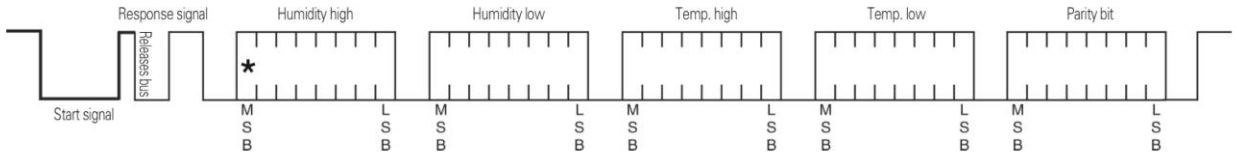
\includegraphics[width=\linewidth]{graphics/DHT22_signal.png}
\caption{Signal of a DHT22 sensor-read as presented in the manual \cite{AM2302}.}
\label{f:dht22_signal}
\end{figure}

\subsection{Gyroscope}
\label{ss:gyro_module}
This module manages the MPU6050 gyroscope and accelerometer.
It is responsible to setup the sensor and report its result.
An implementation for the MPU6050 was present in the nRF52 15.3.0 SDK, but is no longer avaliable for the nRF52 17.1.0 SDK, used in this project.
The old implementation was ported to this project.
This consisted of replacing deprecated parts of the SDK with updated ones and adding newly required flags to the build.


MPU6050 sensors use the I2C communication protocol.
The nRF52 SDK does not include an implementation for this protocol, but has a Two Wire Interface (TWI) implementation that is compatible with the I2C protocol.
During startup the TWI module has to be initialized.
This is handled by the SDK, but requires some parameters to be passed.
\begin{itemize}
	\item The Serial Clock Line (SCL) defines what pin will be used for the clock shared in the TWI. This implementation uses pin 11.
	\item The Serial Data Line (SDA) defines which pin is used for the data communication. Pin 12 was used.
	\item The frequency which the TWI uses. It is defined in MPU6050 data sheet, and is 100 kHz \cite{MPU6050}.
	\item The Interrupt priority is a rank that determins, how easyely this process can cause an interrupt. It is set to high.
\end{itemize}
After the TWI service is initiated with these parameters, it is enabled, ensuring that its resources are locked and can not be used by other services.


Afterwards the results from the sensor can be read using the TWI service again.
The TWI-TX requires the adress of the read device and a registry where to write the MPU6050 datasheet \cite{MPU6050}.
The adress of the sensor is the same for all MPU6050 sensors and can be found in the manua
It sets a flag to true once the sensor has writen the data, which then can be read using the TWO-RX function.
The result consist of three 16-bit integers, representing the angular velocity arround the X,Y and Z axis, shown in figure \ref{f:MPU6050_orientation}.\\
Returning this data when queried has only limited use.
It represents a measurement of the current situation.
The caller is more interested what happened since the last query.
Two different implementations for the read of the gyroscope were used during the experimental phase of this thesis.
One would try to return the current orientation of the tag. This read will be called the \textit{orientational read}.
The other would return the maximal registered angular velocity since the last read. This will be called the \textit{angular velocity read}.


\begin{figure}[ht!]
\centering
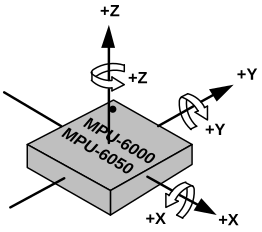
\includegraphics[width=200px]{graphics/MPU6050_orientation.png}
\caption{Schematic view of the MPU6050, showing the direction of the three axis X,Y,Z.}
\label{f:MPU6050_orientation}
\end{figure}



To achieve the orientational read, three orientational variables $x_{angle}$, $y_{angle}$ and $z_{angle}$ keep track of the current rotation around their corresponding axes.
During setup, all three angles are set to zero.
The MPU6050 is read out periodically in between calls.
The elapsed time since the last read is multiplied with the angular velocity at this moment arround the axis and is added to the orientational variables.
When the gyroscope module is queried for its measurement, $x_{angle}$, $y_{angle}$ and $z_{angle}$ are returned.


The angualr velocity read is achieved in a similar manner.
Three angular velocity variables $x_{max}$, $y_{max}$ and $z_{max}$ are created and set to zero during initiation.
The MPU6050 is read out periodically and its values are compared to the angular velocity variables.
If any of the angular velocity values is smaller in absolute magnitude than the corresponding read value, it is replaced by that read value.
When the the gyroscope module is queried, the values of $x_{max}$, $y_{max}$ and $z_{max}$ are returned.
The angular velocity variables $x_{max}$, $y_{max}$ and $z_{max}$ are then set to zero again.

\subsection{Network}
\label{s:network}
The network module is responsible for the managment of the network.
This consists of: sending requests to join a network, managing requests to join a network, keeping track of its neighbours, transmitting messages and sending messages.
Since only four devices were used in this implementation, the processes for the network are much more simplified, then presented in design chapter.
A 4-connected minial graph of 4 verteces must nececarily include that all the nodes are fully connected.
This leads to a simplified network architecture.
Since this implementation was build to run experiments and not to be used in real-world applications, a lot of security measures were canceled.
Messages are not encrypted and devices are not authenticated.
All messages are assumed to reach their destination and no devices is expected to become unavaliable. \\
The Network-module is based on the implementation of \cite{degkwitz2023ultrawideband}.
It is based on published examples from Qorvo, the producer of the DWM3000 shield.
It uses the DWS3000 SDK to communicate with the DWM3000.


The DWM3000 uses the Serial Peripheral Interface (SPI) protocol.
This requires some resources that have to be reserved and some configurations that need to be set.
This is the first thing that happens during the setup of the UWB network.
Next the interrupt-priorities and the communication speed of the SPI connection are configured.
Then the DWM3000 is reset, to insure no cross-effects from previous sessions are possible.
Then the board is told to initialize.
After that the used configurations are send to the shield.
This includes information like chanel number, preamble codes, data rates and header modes.
The SDK contains many pre-defined configurations.
All configurations that allow for RX and TX and that use scrambled timestampt (STS) work for this usecase.
It is crucal that all tags use the same configurations.
For this implementation the same configurations were used, as in \cite{degkwitz2023ultrawideband}.
The configurations can be seen in table \ref{table:DWM_settings}.
The setup finishes with initiating the LEDs, that serve no critical service, but are usefull for debugging.



\begin{figure}[ht]
\caption{Configurations of the DWM3000 for UWB communication}
\begin{longtable}{|l|c|}
\hline
\textbf{Description} & \textbf{Value} \\
\hline
\endfirsthead
\hline
\endfoot
Channel number & 5 \\
TX preamble length & 128 symbols \\
RX preamble acquisition chunk size & 8 chunks \\
TX preamble code & 9 \\
RX preamble code & 9 \\
SFD type selection & 4z 8 symbol\\
Data rate & 6.8 Mbits/s \\
PHY header mode & standard PHR mode \\
PHY header rate & standard PHR rate \\
SFD timeout & 129 \\
STS mode & enabled \\
STS length & 128 bits \\
PDOA mode & off \\
\hline
\end{longtable}
\label{table:DWM_settings}
\end{figure}


The Certify project uses unique, falsifiable identifiers for its tags.
Since this is not avaliable for the tags used here, the device-ID was used instead.
It serves as a 8-bit long adress for the purposes of this implementation.
Each tag also keeps a list of all known adresses, called neighbours.


The adress \textit{0x3F} was used, when a tag wants to join a network.
This was chosen since none of the used devixes had this device-ID, and it corresponds to a question mark when using ASCI encoding.
When a tag wants to joind a message, it sends the adress \textit{0x3F}, followed by the message 'findnet', and its own adress.
It then start listening for answers.
If the listening timed out without any answers, it sends the message again.


For the network to function, the receiving and sending of messages is critical.
The UWB listener function from project \cite{degkwitz2023ultrawideband} was modified.
It waits for a listened message from the shield.
If it receives a message, it coppies it to a buffer.
It then checks the first bit of the message for the receiver adress.
If the receiver adress is equivalent to the tags own adress, it passes the message on to the job-handler module for further evaluation.
Otherwise the message is discarded.
An exception is made, if the receiver-adress is "\textit{0x3F}", indicating that a tag is looking for a network.
In that case, the network module adds the tag to the list of neighbours.
It then waits for a time proportional to its own adress, before continuing.
Since adresses are unique, this ensures that no two tags responde to the new tag at the same time.
Afterwards it sends a new message, beginning with the adress of the new tag, followed by the string 'NEW' and its own adress.
This way it can be added to the neighbours of the new tag as well.\\
For sending messages, the implementation of \cite{degkwitz2023ultrawideband} was modified.
It sets the DWM3000 to TX, passes a int-buffer and lets it transmit, before returning to RX mode.
Do to limitations discussed in section \ref{ss:combination}, the message length could not exceed 10 bytes. 


\subsection{Two-way ranging}
\label{ss:two_way_ranging}
The two-way ranging module is responsible for measuring its distances to the tags in the neighbourhood.
Since it also uses the DWM3000 shield, it requires no additional setup.


When the two way ranging module gets a distance request, it loops over the list of neighbours, performing two-way ranging with each of them.
First it sends a prepare-rainging request to the neighbour it wants to performe ranging with, before performing the ranging.
It then sends the result back over the network to the requesting tag with the following format: 
\begin{equation}
	\mbox{$a_r$DST$a_ta_ncd_{tn}$}
\end{equation}
with
\begin{itemize}
	\item $a_r$: The adress of the requesting tag.
	\item DST: The string "DST", indicating the purpose of the message.
	\item $a_t$: The own adress of the tag performing the measurement.
	\item $a_n$: The adress of the neighbour that the distance was measured to.
	\item $c$: A boolean. If false, this is the last neighbout measured for this query.
	\item $d_{tn}$: The distance to measured. 
\end{itemize}
The reason for each measurement triggering its own response is the message-lenght limitation mentioned in section \ref{s:network}.

When a tag receives a prepare-rainging request intended for another device, it enters a short sleep.
This is because rainging envolves multiple messages beeing send netween both participants.
This would unnecesarily drain energy from the tags that are not envolved.
Because of that they sleep for the expected duration. \\
If the tag is the entended receiver for the prepare-rainging message, it will enter the preparation part of the two-way ranging module.
If will function as deivce A in respect to figure \ref{f:ds_twr_3}.
In a first step, it will clear all RX and TX buffers.
It then sets the expected RT and TX antenna delays, $d_{rx}$ and $d_{tx}$.
They represent the expected time loss during receiving or transmitting messages and are device specific.
These delays will automatically be taken into account, when calculating the timestamps.
It then sends the first polling message and imideatly starts waiting for a response.
The polling message is a constant string with no changing data.
The DWM3000 will automatically store the transmission and reception timestamps, their is no need to retreive it right away.
When the response is received, it checks if it is the expected response.
If it is, the two timestamps $T_{TX_1}^A$ and $T_{RX}^A$ are retireved.
The final transmission time $T_{TX_2}^A$ is calculated by adding a constant $c_A$ to $T_{RX}^A$:\begin{equation}
	\mbox{$T_{TX_2}^A$=}
	\mbox{$T_{RX}^A+c_A$}
\end{equation}
The final message is then prepared, containing all three timestamps $T_{TX_1}^A$, $T_{RX}^A$ and $T_{TX_2}^A$.
The message is loaded into the message buffer of the DWM3000 and a delayed transmission is started.
The delayed tranmission takes the timestamp $T_{TX_2}^A$ and will start the transmission once that timestamp is reached.
Afterwards all caches are cleaned and the tag returns to its previous state, listening for requests.

The tag that performs the ranging roccesponds to device B in figure \ref{f:ds_twr_3}.
Once it has sent the the prepare-rainging message to its neighbour, it will enter the revceiving part of the two-way ranging module.
As device A, device B will also start by settings its antenna delays $d_{rx}$ and $d_{tx}$ and clear all its RX and TX buffers.
It will then start polling for a message.
Once a message from device A is received and validated, it will retreive the timestamp when the message was received, $T_{RX_1}^B$.
Device B will add a constant $c_B$ to this timestamp to get $T_{TX}^B$:
\begin{equation}
	\mbox{$T_{TX}^B$=}
	\mbox{$T_{RX_1}^B+c_B$}
\end{equation}
It will then start a delayed transmission for the response message at $T_{TX}^B$.
The response is a constant string without any data.
Once the response is sent, device B starts to listen for messages again.
When the final message is received from device A and validated, $T_{TX_1}^A$, $T_{RX}^A$ and $T_{TX_2}^A$ are extracted from the message.
Device B also retreives its final timestamp, $T_{RX_2}^B$.
Once this is done, the time of flight for a single message can be calculated, and from that the distance:
\begin{align}
    T_{round1} &= (T_{RX}^A - T_{TX_1}^A) \\
    T_{round2} &= (T_{RX_2}^B - T_{TX}^B) \\
    T_{reply1} &= (T_{TX}^B - T_{RX_1}^B) \\
    T_{reply2} &= (T_{TX_2}^A - T_{RX}^A) \\
    ToF^{AB} &= \frac{(T_{round1}\cdot T_{round2}) - (T_{reply1}\cdot T_{reply2})}{T_{round1} + T_{round2}) + (T_{reply1} + T_{reply2}} \\
    distance &= ToF^{AB} \cdot c_{air}
\end{align}
The distance is then returned, all caches cleared and the module continues with the next distance measurent, if any are remaining.


The TX and RX antenna delay $d_{rx}$, $d_{tx}$ are different for each device.
Qorvo supplies a default value, but it is the same on all devices.
Since te antenna delays are multiplied with the speed of light, even small mistakes in calibration can lead to big errors.
According to qorvo, without the calibration of antenna delays, a measurement can be off by up to 40 cm \cite{DWM3000Calib}.
This will be a constant bias and not change over measurements.\\
Qorov has published a manual on how to calibrate their devices \cite{DWM3000Calib}.
They have not published a codebasis that implements this process.
The calibration process published by Qorvo required things that were not part of this project:
\begin{itemize}
	\item A synchronized clock, shared over all devices, without significant clockdrift
	\item A UART connection to a computer
	\item A pipeline performing statistical analysis and coordinating the devices.
\end{itemize} 
Since implementing this calibration process whould have been out of scope for this thesis, a simpler version was designed.
The tags were set up in a theathedron, so each tag was 30 cm apart from each other.
Then one tag would perform two way ranging with another tag, chosen at random.
The result would be shared between both tags.
If the result was larger than 30 cm, $d_{rx}$ or $d_{tx}$ would be chosen at random and increased.
If it was lower, $d_{rx}$ or $d_{tx}$ would be increased.
Then the second tag would start a new ranging session with a random tag.
This system was left running for over one hour, until all distances measured were in the range of [27 cm, 33 cm].


\subsection{BLE}
\label{ss:ble_module}
The BLE module is responsible for the communication between the UWB network and the phone.
It advertises the tag to the phone and receives messages from the phone and sends messages to the phone using BLE.
The nRF52840 microcontoler is equiped with a antenna with BLE capabilities.
The nRF52 SDK includes libraries for the managment of this antenna.
It also includes the \textit{ble{\_}app{\_}uart} example project.
This project offers advertises a ble connection, handles the paring process.
Once connected, it forwards all incomming comunication to a USB-UART mdoule connected to a computer.
Input from the computer ver USB-UART is sent as a message to the paired device.
The  \textit{ble{\_}app{\_}uart} example project was took as a basis to build the BLE-module.


The nRF52 SDK for BLE requires the use of the S140 SoftDevice.
The S140 SoftDevice is a BLE protocol stack that can be used for the 811, 820, 833 and 840 series of nRF52 boards.
In order for the SoftDevice to be avaliable, a memory 156 kilobyte segment of memory has to be reserved for it, starting at  memory segment 0x0.
The SoftDevice then has to be flashed to the board.

During startup, the BLE module has to initialize a few services and reserve some resources.
Firstly a nRF clock has to be reserved for the BLE module.
Then the powermanagment for the SoftDevice has to be initiated, before the BLE stack inside the SoftDevice can be initialized.
Next the Generic Access Profile (GAP) and the Generic Attribute Profile (GATT) have to be prepared.
The information what functions to call when the SoftDevice receives data has to be set, as well as the advertized name, the UUID, timeout durations and what to do on faults.
The advertized name was left unchanged from the \textit{ble{\_}app{\_}uart} example, "Nordic{\_}UART".\\
Once the SoftDevice is initialized and the tag has connecteced to the UWB network, the BLE connection can be advertized.
The avertisement function of the nRF52 SDK was used for this.


The BLE module listens for queries sent from the Phone to the tag using BLE.
To achiev this, a query-handler function was passed to the SoftDevice during initiation.
All incomming messages will be passed to this function by the SoftDevice.
When a query is received, the BLE module interprets the message.
It checks what is beeing queried and transformes it into a job, readable by the Job Handler module.
The BLE module also offers a service to send messages to the phone.
This service uses the nRF52 SDK to load the message into a the SoftDevice and send it to the phone.


\subsection{Job Handler}
\label{ss:job_handler_module}

The job-handler module connects all other module.
It takes job structs (see figure \ref{code:job_struct}, interprets which module is responsible for handeling them and calles the job together with the relevant data.
The job struct consits of a field for the job-type, that tells the job-handler what type of job this is. It also includes fields to store data, that is needed for the job.

\begin{figure}[h]
    \centering
    \begin{lstlisting}[language=c]
    struct job {
  		enum job_types type;
  		uint8_t* data;
  		int length;
};
    \end{lstlisting}
    \caption{Job struct}
	\label{code:job_struct}
\end{figure}

There are 14 total job types.The following list while decribe the meaning of them, as well as how they are handled by the job-handler:
\begin{itemize}
  \item \textbf{search for network}: This job is triggered after setup. The tag is not connected to the network. It will be passed to the Network module without any aditinal data.
  \item \textbf{join network request}: This job commes from the Network module, when it receives a request from another tag to join the network. It will be passed back to the Network module, with the data of the new devices id.
  \item \textbf{set network and address}: This job commes from the Network module. It informs the network connection has been established. The job is handed back to the Network module, with the received message, to be added to the list of neighbours.
  \item \textbf{ble temp hum request}: This job commes from the BLE module, where a query for temperature and humidity has been registered. The requested tag is extracted from the job. If the request is for this tag, the job is handed to the Temperature and Humidity module. Otherwise it is passed to the network module, to be transmitted to the requested tag.
  \item \textbf{temp hum request }: This job commes from the Network module and informs that a request for a temperature and humidity read has been made. It is passed to the Temperature and Humidity module, together with the requesting tags adress.
  \item \textbf{temp hum answer}: This job commes from the Network module and carries the respons to a temperature and humidity request. It is passed to the BLE module, togehter with the measurement, which will be passed to the phone.
  \item \textbf{ble gyro request}: This follows the same logic as "ble temp hum request", but with the gyroscope module.
  \item \textbf{gyro request}:This follows the same logic as "temp hum request", but with the gyroscope module.
  \item \textbf{gyro answer}:This follows the same logic as "temp hum answer"
  \item \textbf{ble distance request}: This job comes from the BLE module. The phone has queried for a distance. If the queried tag is not this tag, the message is passed to the Network module. Otherwise, it is passed to the Two-Way Ranging module.
  \item \textbf{distances reques}: This job comes from the Network Module. It requests a distance measurement. The job is passed to the Two-Way Ranging module, together with the requeting tags adress.
  \item \textbf{distances prepare}: This job comes from the Network Module. It informs, that another tag is requesting a ranging session. If the ranging session is with this tag, the job is passed to the Two-Way Ranging module. Otherwise the tag goes to sleep for a short time.
  \item \textbf{distances answer}: This job comes from the Network module. It reports that a distance measurement as been returned. The job is handed ober to the BLE module, together with the content of the message.
  \item \textbf{ble get known devices}: This job comes from the BLE module. It requests a list of all neighbours. The job is transfered to the Network-Module.
\end{itemize}


\subsection{Combining modules}
\label{ss:combination}
Each module except for the job-handler module was developed in seperate projects, to ensure operability.
Afterwards the modules were merged into one project.
The Network module was chosen as the base project, that the other projects were merged into.
This was chosen since the Network module was based on \cite{degkwitz2023ultrawideband}, which intern was based on a example published by Qorvo.
The Qorvo example uses a lot of shorthand, magic numbers and development shortcut, that are not easely readable to developers outside the firm.
The Network module whas therefore chosen as a basis, since merging it into another project would likely be cumbersome, since parts would easely be forgotten or interact poorly, without the knowledge or udnerstanding of the developer.
Combining the modules came with several chalanges, that described in this section.


The Qorvo example that builds the basis of the Network module uses the pin-mapping PCA10056.
This is the pin mapping for boards that include the NRF52840 board, but not the NRF52840 development board, that this example was made for and is used in this thesis.
The NRF52840 board does not contain the nesecary pins to attack a DWM3000 board to it.
This wrong pin-mapping leads to mistakes that the Qorvo example has to work around.\\
When switching to the correct pin-mapping, PCA10040, the Network mdoule would no longer work, since those work-arounds now introduced mistakes now.
Sice fixing the Qorvo example code would have been cumbersome, it was decided to instead change the other modules that used pins, the Gyroscope module and the Themperature and Humidity module.
The pins for those modules, pin 11, 13, and 13. where hard coded into the modules, instead of using the pin-mapping.


The nRF52 SDK offers a rich selection of tools, such as SPI and TWI communication, clocks, ble capabilities, SoftDevice, UUIDs.
These tools are all enabled or disbaled in the sdk{\_}config file.
Merging in general requires only to enable the tools needed by the merged module.\\
Three mdoules requie a nRF clock,, Two-Way Ranging, Temperature and BLE.
The nRF SDK offers  exactly three clcoks slots, so all of them have to be enabled with the apropriate clock type.
Each module has to be adapted, so it uses its assigned clock-slot. \\
The nRF52 SDK can suport up to three SPI or TWI conenctions simultaniosly, nemaed SPI0, SPI1, SPI2, TWI1,TWI2 and TWI3.
SPI and TWI share their memory, so SPI0 can not be used while TWI0 is used and vise-versa.
Since the DWM3000 uses two SPI connections and the MPU6050 uses one TWI connection, exactly enough resources remain, for both devices to run simultanisously.
SPI0 and SPI1 were used for the DWM3000 and TWI3 for the MPU6050.\\
All other SDK resources were non-conflicting.
They were ported from the original module implementation to the merged one without change.


As most embeded systems do, the nRF52840 requires static memory allocation during flashing.
The avaliable memory is seperated into flash-memory and random-access-memory (RAM).
Some memory segments are required by every runable system:
\begin{itemize}
	\item FLASH, \textbf{vectors}: The interrupt vector table defines the interrput handlers for the system, like resets, faults.
	\item FLASH, \textbf{init}: The initialization routine sets up clocks, pins and other peripherals.
	\item FLASH, \textbf{text}: This section contains the executable code in mashine language.
	\item FLASH, \textbf{data}: This section contains the initial values for all global values..
	\item \textbf{rodata}: This section contains the constant variables, that will not change at runtime.
	\item RAM, \textbf{data}: During startup, the initial values for changable global variables are coppied to this section. They can change at runtime.
	\item RAM, \textbf{bss}: This section contains the global variables that do not have initial values.
	\item RAM, \textbf{stack} and \textbf{heap}: The stack and heap that build the runntime environment.
\end{itemize}
Neither the MPU6050 nor the DHT22 require any additional memory segments.
The DWM3000 and the BLE module both require additional memory segments. \\
The BLE module reuqires the SoftDevice to be added to memory. The Softdevice requires 156 KB of Flash and 10.7 KB of RAM.Those reserved memory segments need to be the first one in both Flash and RAM. This additionaly requires SoftDevice oberservers for System on Chip (SoC), BLE, state and stack. Additionaly a segment to house the nRF52 SDK memory allocator is required, nrf{\_}balloc. These segments are rather small, never exceeding 32 bytes.\\
The DWM3000 shield requires two additional memory segments, fConfig in Flash and nrf{\_}balloc in RAM. 
Qorvo does not publish what the fConfig module is for, but it is required for the shield to work. \\
Since the base project was made for the DWM3000 shield, it had to be addapted to addinionaly fit the segments needed for the BLE module. This mainly consisted of moving all segments to later adress-spaces to add room for the SoftDevice reserved memory. All other memory segments had to be added as well. To make room for this, the Flash memory had to be expanded. \\
The Qorvo example implementation for the DWM3000 shield uses some work-arrounds. An example of this is the "NRFX{\_}SPIM3{\_}NRF52840{\_}ANOMALY{\_}198{\_}WORKAROUND{\_}ENABLED" present in the SDF configuration. These workarounds let the SPI communication with the shield perform certen memory manipulation. If these workarounds are necessary is doubtfull, but fixing them would have been out of scope for this thesis.
The workarounds do generaly have no effect on the implementation, with one excpetion. When the DWM3000 receiver sends a message longer than 10 bytes to the microcontroler over SPI, it incroaches on the SoftDevice RAM. This behaviour was found experimentaly, the responsible code could not be located. Since the system can be implemented with the restriction of 10 byte messages, this was done.



\section{App}
\label{s:app}
Nordic Semi Conductors, the maker of the used microcontrolers, published the code to a simple app that allows for BLE communication with their devices.
It is called nRF Toolbox.
It is intended to pair with the \textit{ble{\_}app{\_}uart} example, published in the nRF52 SDK.
Since this example code was used as the basis for the ble communication used in this project, it was addapted to work with this project.


The App contains different modules, intended for different examples, among them the Universal Asynchronus Receiver/Transmitter (UART) module (see \ref{f:Toolbox_modules}).
It is intended to be used with the ble\_ app\_ uart example.
When opem it shows the ble services that are currently beeing addvertised and allows the user to connect to one of them \ref{f:Toolbox_connect}.
It then opens a window similar to phone messangers, were the keyboard can be used to tpye messages, that are sent to the connected devices.

\begin{figure}[ht!]
\centering
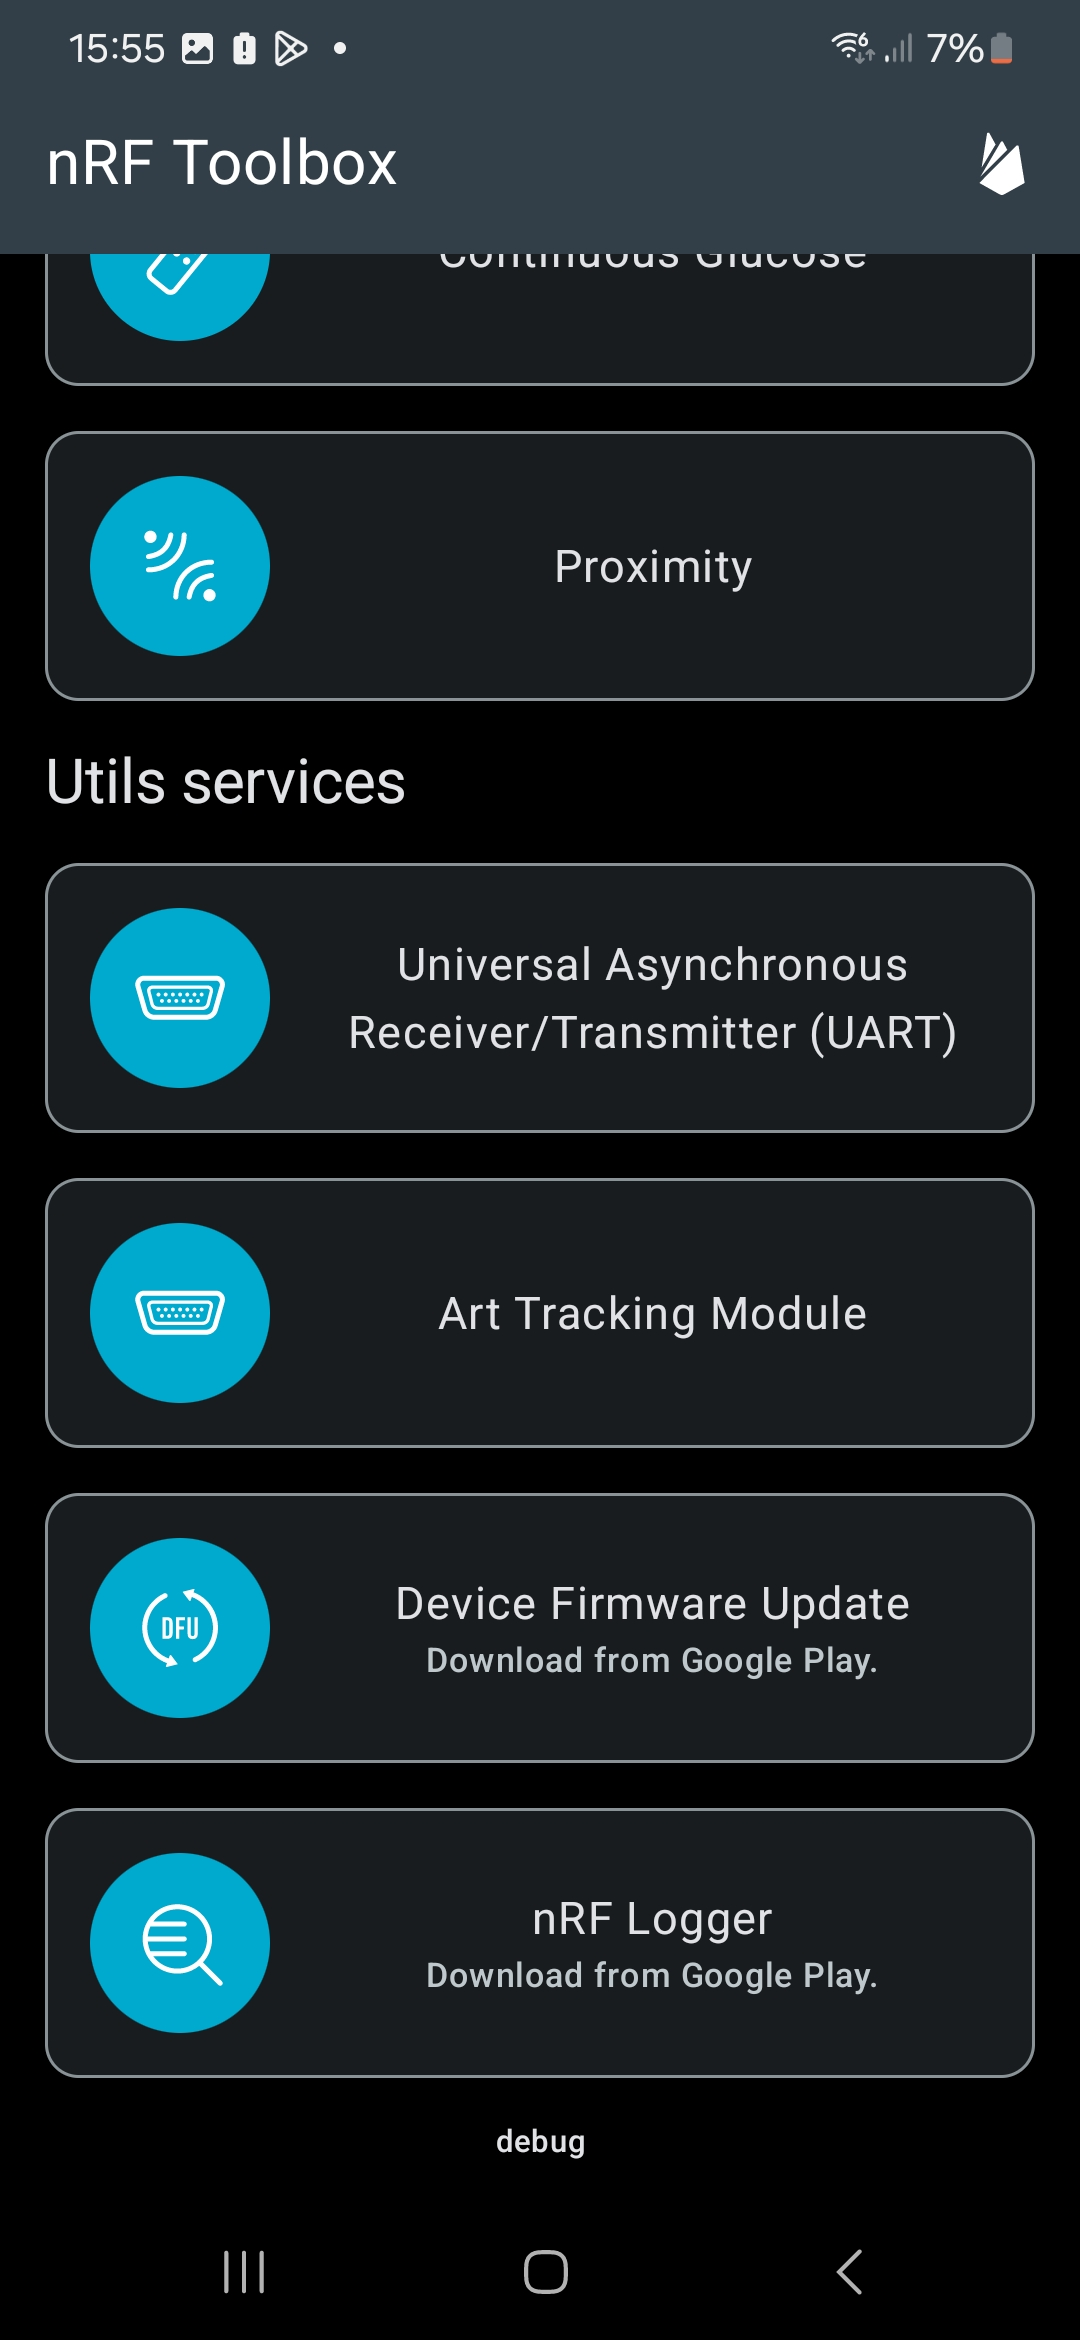
\includegraphics[width=200px]{graphics/nRF_toolbox_modules.jpg}
\caption{nRF Toolbox module menue, with the added Art Tracking Module}
\label{f:Toolbox_modules}
\end{figure}

\begin{figure}[ht!]
\centering
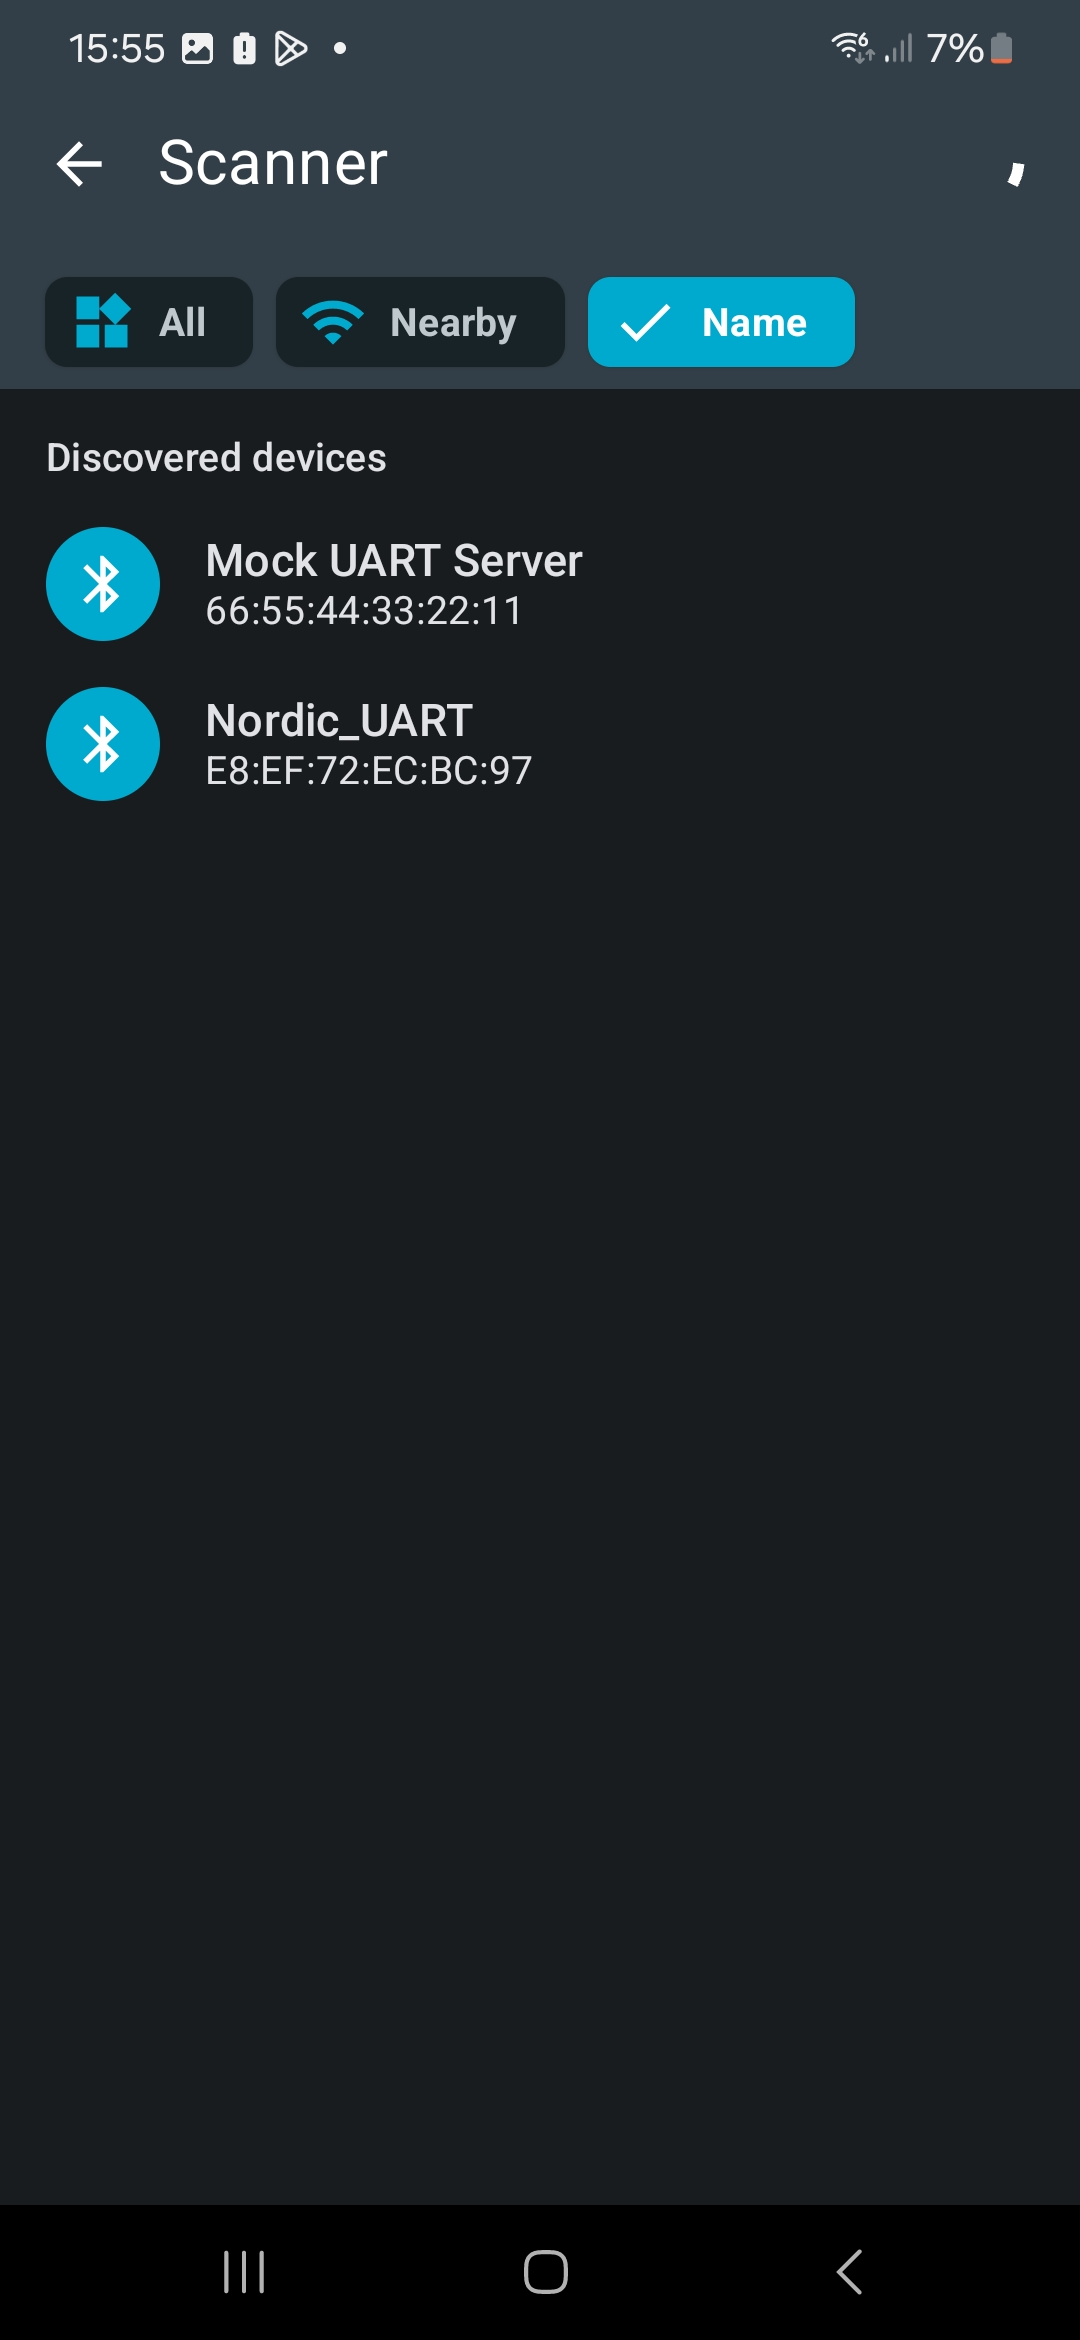
\includegraphics[width=200px]{graphics/nRF_toolbox_connect.jpg}
 \caption{nRF Toolbox shows avaliable devices to connect to}
\label{f:Toolbox_connect}
\end{figure}

\begin{figure}[ht!]
\centering
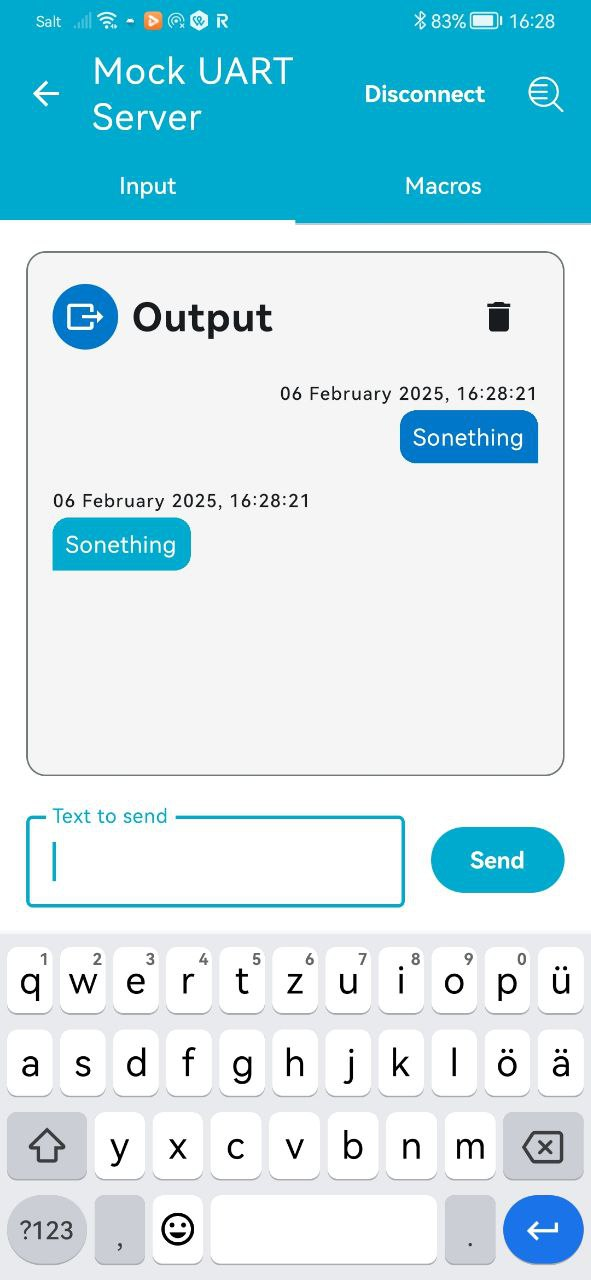
\includegraphics[width=200px]{graphics/nRF_toolbox_messanger.jpg}
\caption{nRF Toolbox UART module screen}
\label{f:Toolbox_output}
\end{figure}

Since the development of an application was not the primary focus of this thesis, it was decided to take the nRF Toolbox app and add a new module for art-traking to it.
The UART module searved as the basis for this new module, since it had a lot of usefull services already implemented.
As with the UART module the art-tracking module opens up the same connection page \ref{f:Toolbox_connect}, that allows the user to select the art-tracking and connect to it.

Once connected, the observation screen is shown (figure \ref{f:Toolbox_art_tracking_empty}).
At the bottom seven parameters can be set: \textit{time}, \textit{max Temp}, \textit{min Temp}, \textit{max Hum}, \textit{min Hum}, \textit{max Angle}, \textit{max Dist}.
The parameters \textit{max}/\textit{min} \textit{Temp}/\textit{Hum} represent the expected range of humidity and temperature.
Any measurement outside these parameter will be considered a dangerous value by the app.
The tollerated difference in angle compared to the previous measurement is set by \textit{max Angle}, larger differences are considered dangerous values.
Distance measurement work analogously with \textit{max Dist} in meters.
The \textit{time} set defines the time that passes enbetween measurements in seconds.
The default is set to 350 seconds.
This means that the time that passes between, for example, the temperature measurements on tag 2 are 350 seconds.


\begin{figure}[ht!]
\centering
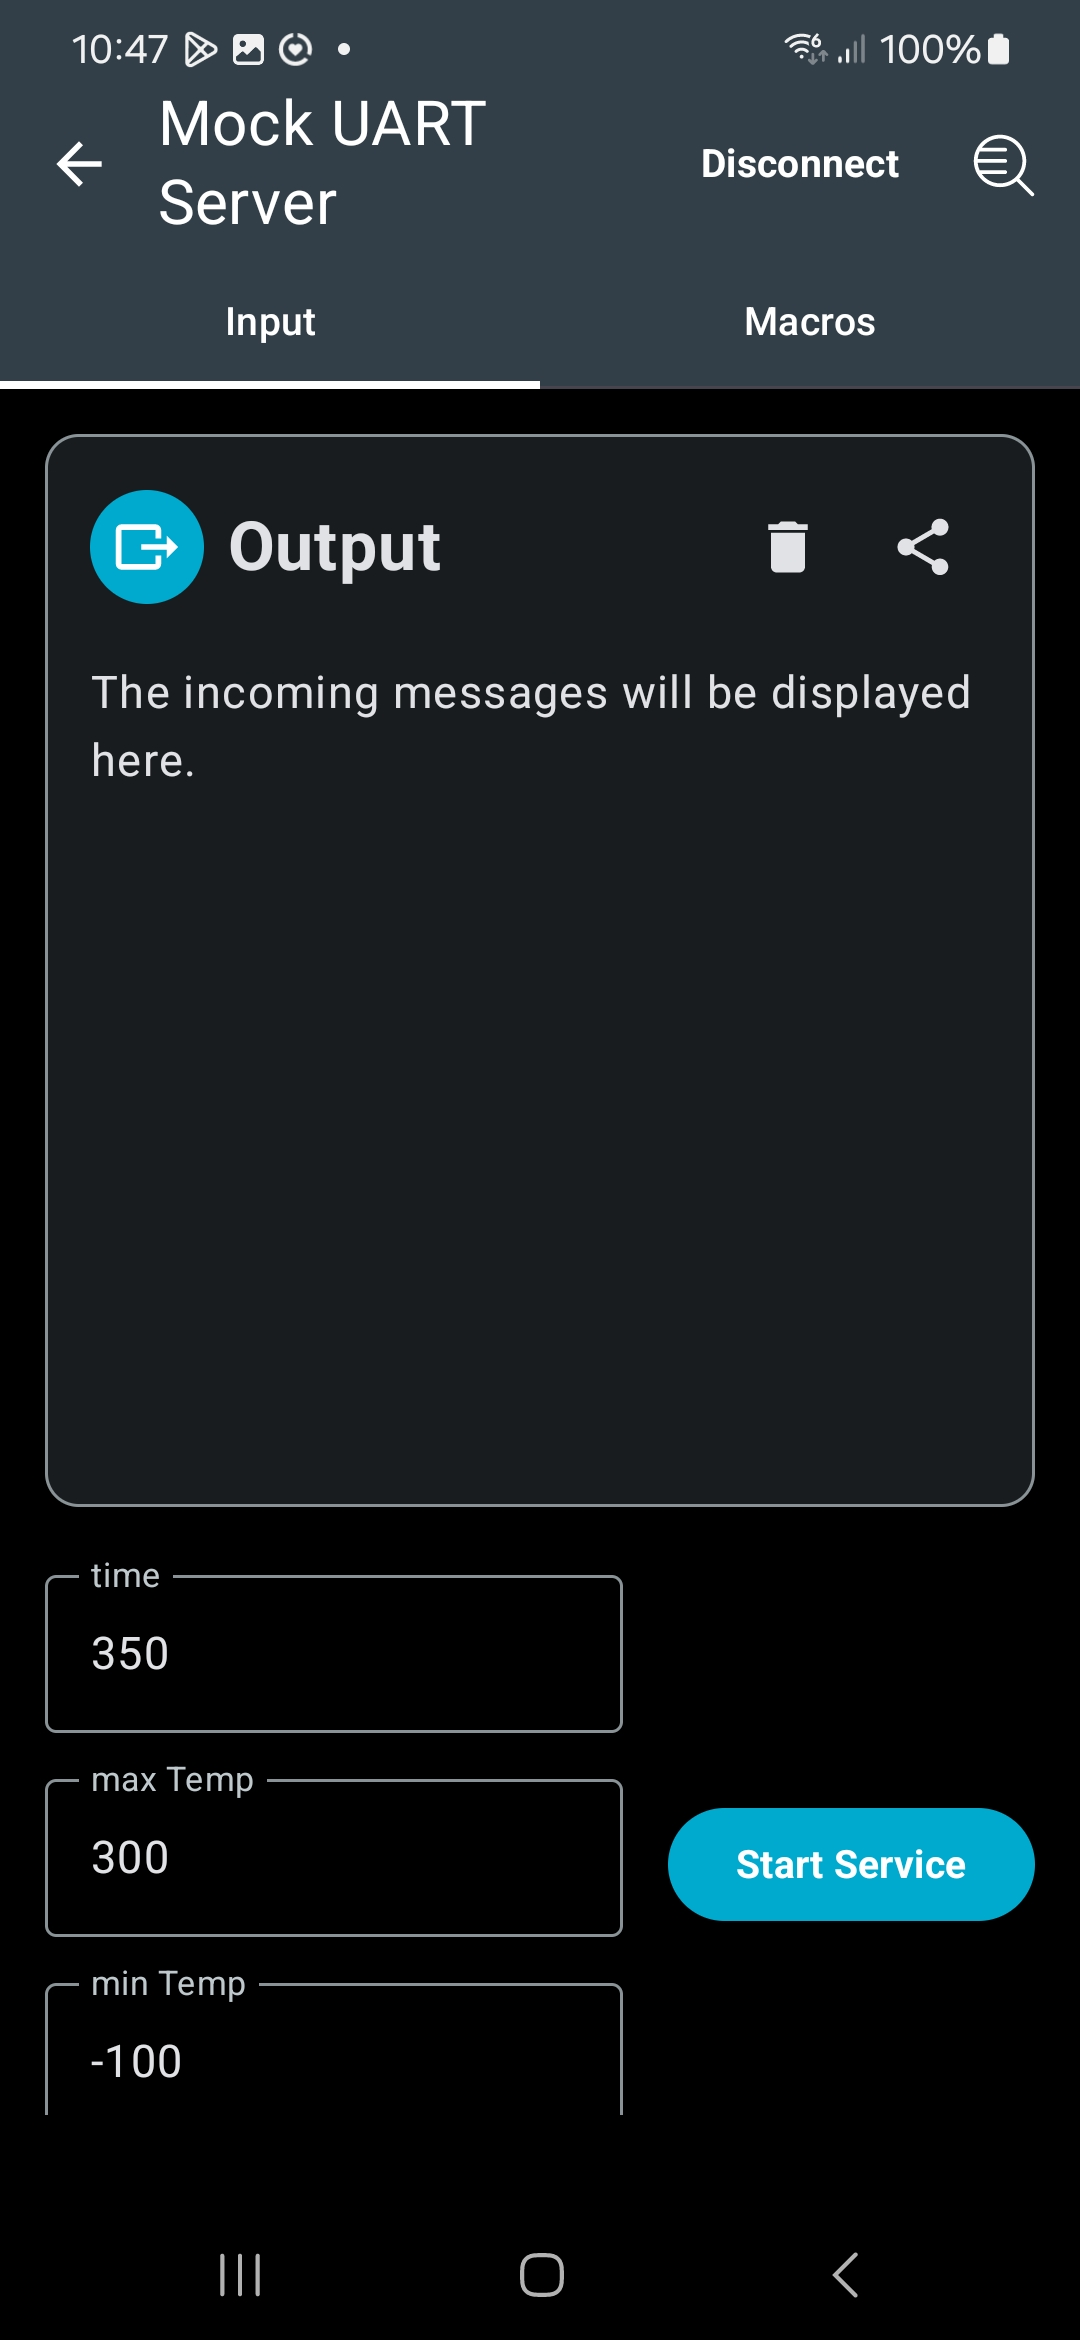
\includegraphics[width=200px]{graphics/nRF_toolbox_art_tracking_empty.jpg}
\caption{Art Tracking module oberservation screen before measurements}
\label{f:Toolbox_art_tracking_empty}
\end{figure}


When the user presses the \textit{Start Service} button, a services starts that poeriodically queries the tags for the Measurements.
Figure \ref{code:App_main_loop} shows the measurement loop.
Each sensor is assigned a character.
\textit{T} for temperature and humidity, \textit{G} for gyro and \textit{D} for distance.
Each tag has a number, here from one to four since four tags were used in the experiments.
The loop concatenates these two characters and sends the resulting query to the connected tag.
Then the next tag-number is prepared for the next query.
Once all tags have been queried for a sensor, the tag-number starts with the first again and the next sensor is queried.
In between cals the app waits.
The call time for distance-measurement is fixed at 80 seconds.
Distance measurement takes longer than the other sensors, since for every devices three measurements need tobe conducted.
Additionaly the sensors that do not participate in a ranging session are sleeping for a quite generous amount of time, to ensure they don't distrub the ranging session.
80 seconds has been chosen, since it allows enough time for all the ranging to happen, plus two repeats per sensor in case the ranging session fails.
For the other sensors the waiting time in between queries is calculated from the remaining set time, after the ranging time is deducted.

\begin{figure}[h]
    \centering
    \begin{lstlisting}[language=Java]
    private val sensors = listOf("T", "G", "D")
    private val devices = listOf("1", "2", "3", "4")
    private var measurement_type = 0
    private var tag = 0
    private var timeBetweenCals: Long = 3750

    private val runnable = object : Runnable {
        override fun run() {
            if (tag >= list2.size) {
                tag = 0
                measurement_type += 1
            }
            if (measurement_type >= list1.size) {
                measurement_type = 0
            }
            val textToSend = "${list1[measurement_type]}${list2[tag]}"
            artRepository.sendText(textToSend, MacroEol.LF)
            tag += 1
            if(list1[measurement_type] == "D"){
                handler.postDelayed(this, 80000)
            } else {
                handler.postDelayed(this, timeBetweenCals)
            }
        }
    }
    \end{lstlisting}
    % Optionally, add a caption to the figure
    \caption{Section from the ArtMetricService.kt, main measurement loop}
	\label{code:App_main_loop}
\end{figure}

Once the process has started, the queries will appear in the chat window on the right side of the screen.
The responses are on the right side, see figure \ref{code:App_main_loop}.
If the response is inside the set parameters, the message bubble will appear blue.
If the measured value is considered a dangerous value, the text bubble will appear red (see figure \ref{f:Toolbox_art_filled}).
Since the message display is programmed in a asynchronus way, it can happen, that the answer to a query appears before the querry itself, if the querried tag is the same as the connected tag.
The service can be stopped by pressing the \textit{start service} button again or by exiting this screen in any way.


\begin{figure}[ht!]
\centering
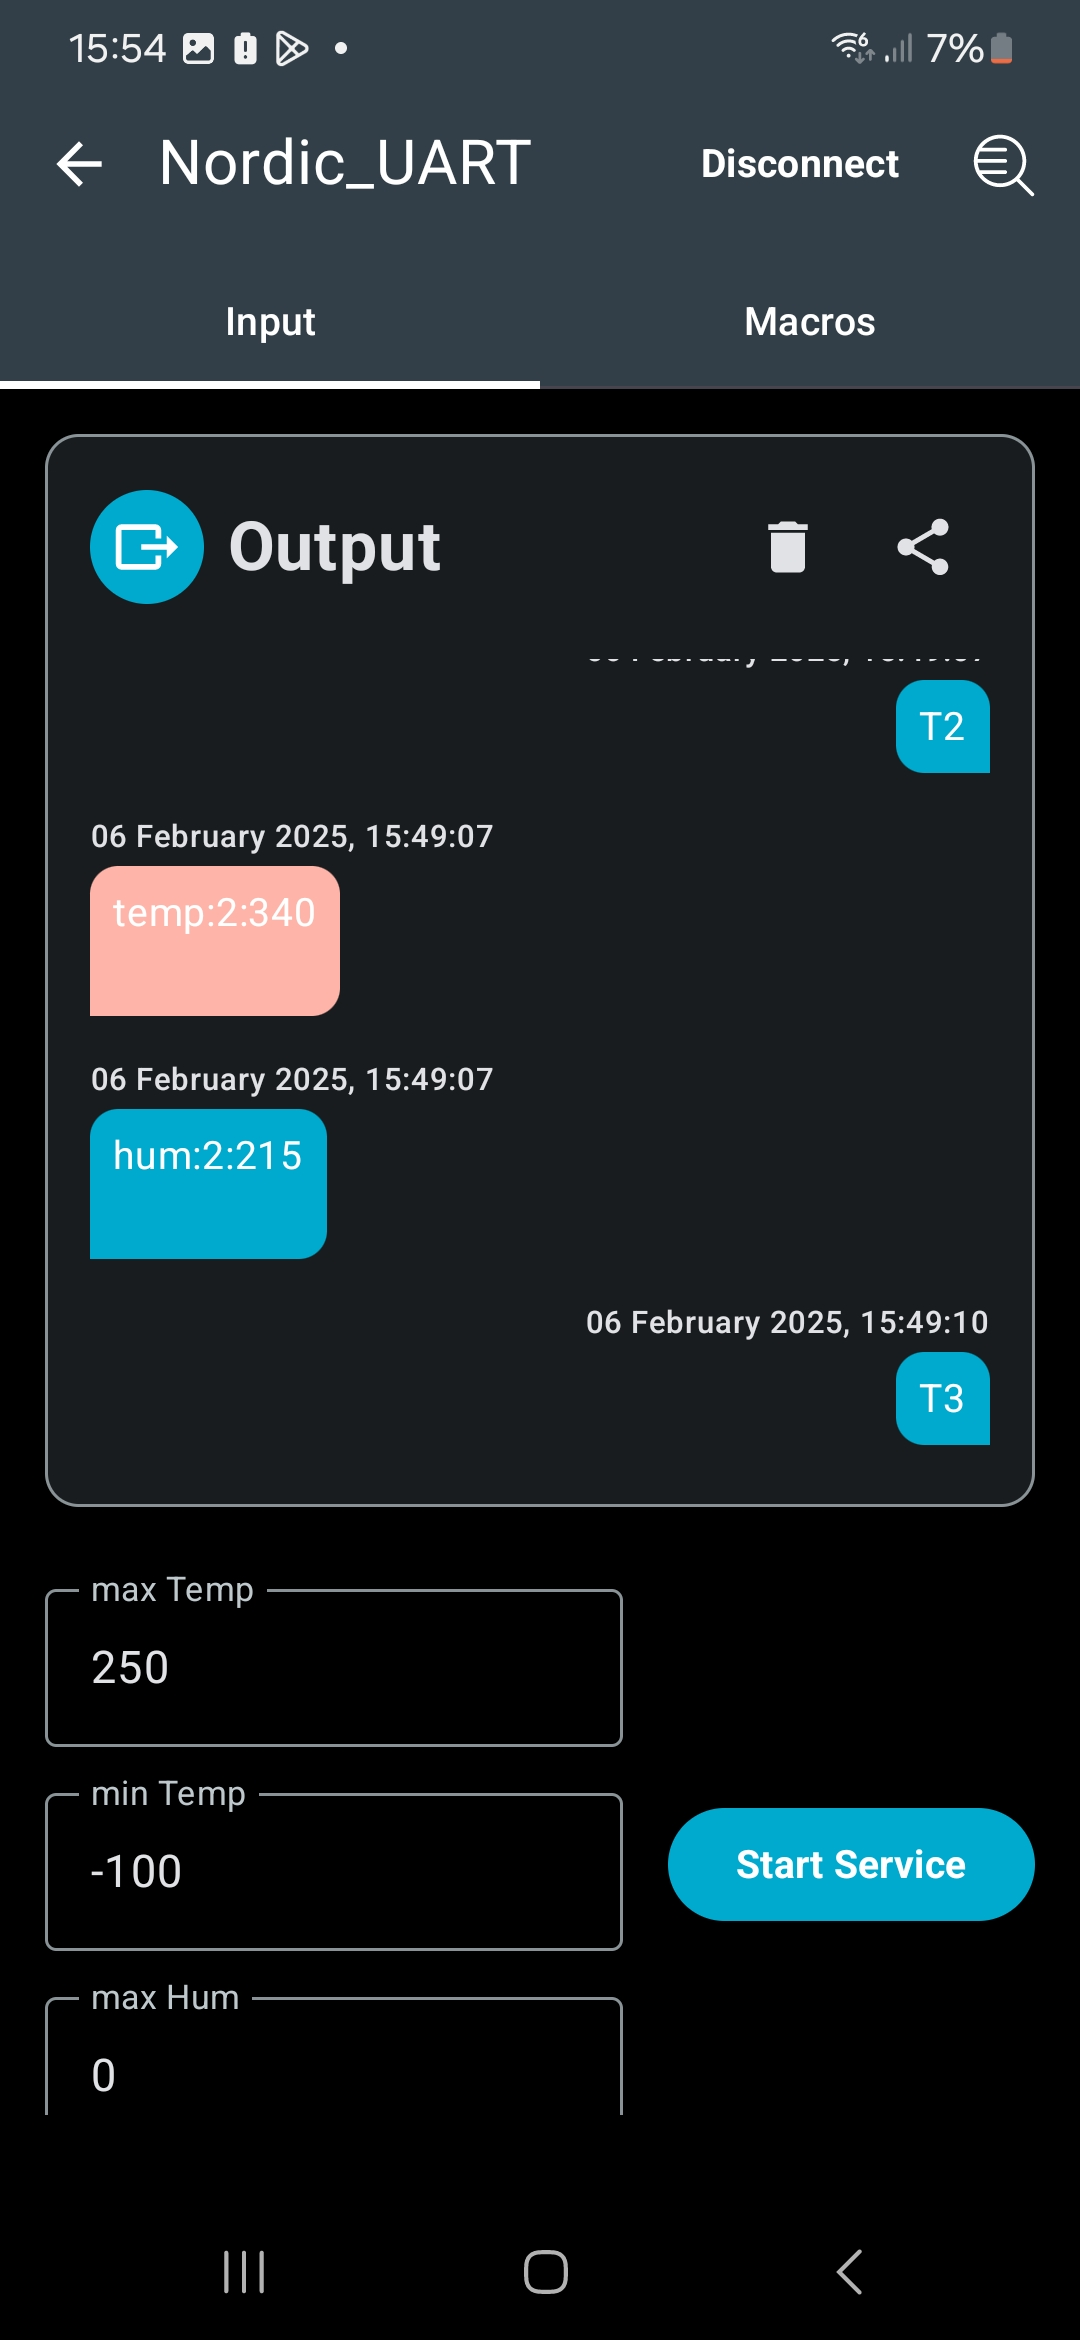
\includegraphics[width=200px]{graphics/nRF_toolbox_Bad_Value_2.jpg}
\caption{Art Tracking module, queries and responses}
\label{f:Toolbox_art_filled}
\end{figure}


%TODO: add image that shows an example file
The query-answers are appended to a file that is safed in the app-storage.
The information appendded consits of: the queried tag, the returned values, a timestamp and if the value was unproblematic.
This functionality is intended for experimental evaluation. 
In a real word application, this data should be periodically backed up on a server in a compressed manner.
When pressing the share-button on the top right of the message-box \ref{f:Toolbox_art_filled}.
It will open the Android naitive share functionality, to share the file over mail, an installed messanger, save it to onedrive or send it over Bluetooth.
In this project all files were sent with email.
Pressing the trashcan next to it will delete the chat and empty the file.
This allows the user to distinguish between different testing session.